\documentclass[12pt,a4paper]{article}

\usepackage[margin=1in]{geometry}

\usepackage[utf8]{inputenc}
\usepackage[T1]{fontenc}
\usepackage{amsmath}
\usepackage{amsfonts}
\usepackage{amssymb}
\usepackage{graphicx}

\graphicspath{{img/}}
\usepackage[numbers, square]{natbib}


\begin{document}

\section{Retinal haemodynamics, vascular disease, neovascular AMD and diabetic retinopathy}

\subsection{Retinal haemodynamics}
\begin{itemize}
\item Intro to what is modeling haemodynamics and the mechanisms at play
\item What diseases and treatment can benefit from modeling this
\item Basis of modelling haemodynamics (i.e. Poiseuille flows, networks, Navier-Stokes, external pressures, Murray's law....)
\end{itemize}
Retinal haemodynamic models are concerned with describing blood flow within the retinal circulation.
Adequate blood flow is essential to ensure delivery of nutrients and oxygen to the retinal cells as well as removing the waste products of those same cells.
Retinal blood flow is controlled by various mechanisms of auto-regulation in order to adapt to changes in the systemic blood flow or in the retinal or choroidal environment.
In response to such changes, retinal vessels can adjust their caliber by making use of a number of communication pathways.
These pathways can be triggered by either a change in metabolic demand of the tissue or variations in pressure.
In particular, vessels are sensitive to variations in the difference between intraocular pressure (IOP) and blood pressure (BP).
Increases in IOP might cause collapse of vessel walls and therefore local shutdowns of blood flow.
Elevated IOP is related with diseases such as glaucoma and retinal vein occlusion. 
Additionally, haemodynamic parameters are direct determinants of oxygen delivery to the tissue.
Therefore, retinal haemodynamic is also relevant to diseases such as neovascular AMD and diabetic retinopathy and other hypoxia-induced disorders. \\
While direct \textit{in vivo} pressure measurements are difficult to achieve, mathematical models can help understand the relationships between retinal haemodynamics and systemic observations (e.g., mean arterial pressure and IOP measurements).
For the most part, those models rely on a framework consisting of:
\begin{itemize}
\item A network of fully connected vascular segments
\item A law describing the viscosity of blood as a function of a vessels diameter
\item A law describing blood flow as a function of viscosity and vessel geometry
\end{itemize}

\subsubsection{Healthy retina}
\begin{itemize}
\item Takahashi's network and distribution of haemodynamics parameters
\item Alletti 2016, transient, Navier-Stokes, fluid-structure interactions
\item Zouache 2015 Choriocapillaris modelling: talk about the missing validation
\end{itemize}

To the best of our knowledge, the first haemodynamic model of the retinal microcirculation is a work done by Takahashi et al.~\cite{Takahashi_2009}.
Their aim was to provide a simple distribution of haemodynamic parameters in the human retinal microvasculature.
In this work, the artiolar tree is approximated by a dichotomous branching tree, with each generation of vessels branching into two vessels, starting from the central retinal artery.
Radius of the daugther vessels is determined by Murray's theoretical law:
\begin{equation}
  \label{eq:MurrayLaw}
  r_p^\gamma = r_{d,1}^\gamma + r_{d,2}^\gamma
\end{equation}
with $r_p$ the parent vessel radius and $r_{d,i},~i=1,2,$ the radius of the daugther vessels~\cite{Murray_1926}.
The exponent $\gamma$ was determined theoretically by Murray to be equal to $3$, however Takahashi et al. used $\gamma=2.85$ as suggested by more recent work.
After branching dichotomously fourteen times, each of the terminal arterioles sprout four capillaries of fixed homogeneous calibre. 
The venous tree symetrically, starting from the central retinal vein to reach the capillary level where both trees are linked together.

Blood is assumed to be an incompressible Newtonian fluid.
Since the vessels are assumed cylindrical and long with a constant cross section for each generation, the Poiseuille law can be used to describe blood flow.
Poiseuille law describes blood flow as proportional to the pressure drop along the vessel by the relation:
\begin{equation}
  \label{eq:PoiseuilleLaw}
  Q = \frac{\pi r^4}{8\mu L}\Delta p
\end{equation}
where $Q$ is the blood flow, $r$ is the vessels radius, $L$ the vessel length, $\mu$ the blood viscosity and $\Delta p$ the pressure drop along the vessel's length.
This approximation fails to work in the smallest calibre vessels of diameter equal or smaller than of the diameter of the red blood cells flowing through them.
As a consequence, vascular resistance is strongly hightened.
To account for this effect, the viscosity of blood is replaced by a varying effective viscosity $\mu_e = \mu_e(r)$ which accounts for this effect and the so-called F\r{a}hr\ae us-Lindqvist effect.
Such viscosity law is only phenomenological and increases viscosity of blood sharply as the vessel radius reaches the size of red blood cells.\\
This work provides an initial estimate of the distribution of haemodynamic parameters in the arterio-venous network in the retina.
It was validated geometrically by comparing the aspect ratio at branches of the arteriolar tree to data from fluorescein photographs of the retina. 
However, it is likely that its efficiency is higher than actual networks since it is generated based on optimality principles and does not include the influence of variying external and internal pressures on the blood flow.
Indeed, several experimental and \textit{in silico} studies have shown that variations in IOP and ocular structure cause strong variations of the haemodynamic of the central retinal artery and, consequently, the downstream vasculature~\cite{Guidoboni_2014, Harris_1996}.

Guidoboni et al. proposed a model that accounts for such variations through a coupling of haemodynamic and mechanistic models of the insertion of the central retinal artery in the retina~\cite{Guidoboni_2014}.
The central retinal artery travels in the optic nerve canal to enter the retina and is subject to to opposite pressures: the cerebrospinal fluid pressure (CRFP) and the intraocular pressure.
Harmful effects of the pressure difference on the central retinal artery are prevented by the lamina cribrosa that surrounds the vessel when crossing the sclera.
By modelling the pressure induced on the vessel, they were able to estimate displacement of the vessel wall along the optic nerve length and the impact on blood flow in the artery in both healthy and elevated IOP conditions.\\
The lamina cribrosa is model as an circular plate.
The plate is subject on its boundaries to stress from the IOP, CRFP and the sclera and is assumed to behave as a nonlinear, homogeneous, isotropic and elastic material.
The resulting stress tensor acts linearly on the outer part of the vessel wall, vessel assumed to be a hollow cylinder passing through the center of the lamina cribrosa.
On the inner surface, the displacement of the wall is provoked by the blood flow within the artery.
Finally, blood flow within the artery is modelled as a Newtonian, incompressible viscous fluid with negligible radial velocity within a cylinder of varying cross section.\\
Across the range of normal intraocular pressures, between $15$ and $20$ mmHg, the model predicted a decrease of almost $5\%$ in blood flow rate.
Variations in the dimension of the sclera and lamina cribrosa can also induce strong reductions of blood flow, particularly in case of elevated IOP. \\


Additionally, as for most vascular beds, retinal vasculature possesses an inherent capacity to regulate blood flow to maintain a near constant blood flow.
This regulation is made possible by the presence of smooth muscle cells on the vessel walls.
These cells are responsible for contraction or dilatation of the vessels in response to changes in the vessel's environment.
Such vascular response may be triggered by variations in systemic blood pressure, metabolic demand, arterial blood gases or intraocular pressure.
By varying the diameter of the lumen, the vasculature is able to increase vascular resistance and reduce or increase blood flow accordingly. 
Failures to maintain retinal blood flow within a healthy range has been associated with a number of retinal and systemic diseases, such as glaucoma, AMD or diabetes~\textbf{Add references (see in DOI: 10.1167/iovs.13-13611)}.
Therefore, it is essential to include autoregulation and the signalling pathways that lead to it in haemodynamic models in order to understand how defects can be an onset of retinal pathologies.\\

In a later paper, Guidoboni et al.~\cite{Guidoboni_2014b} built up on this model of the central retinal artery by including arterioles, capillaries, venules and up to the central retinal vein.
This 0-dimensional model uses the network proposed by Takahashi et al.~\cite{Takahashi_2009}, aggregated into compartments for arterioles, capillary, venules and central retinal vein.
Following an analogy with electrical circuits, different resistances and capacitors properties apply for each compartment.
These properties of electrical circuit represent the vascular resistance opposing the flow and the capacity to store blood volumes and deform.
Applying Ohm's law to the network results in a system of ordinary differential equations involving the time derivatives of transmural pressure in each compartment.
The time dependence comes from the varying systemic arterial pressure which feeds the central retinal artery.
Both a passive and active mechanism of blood flow regulation are introduced in this model through variable resistances.
First, the vascular resistance of a given compartment vary in a passive way through deformation caused by the transmural pressure $\Delta P$ according to:
\begin{equation}
  \label{eq:PassiveVariableResistance}
  R = \frac{8\pi\mu L}{A^2_{ref}}\left(1+\frac{\Delta P}{k_pk_L}\right)^{-4},
\end{equation}
where $A_ref$ is the reference cross section area of the vessel when $\Delta P = 0$, $L$ is the length of the vessel and $k_p,~k_L$ are coefficient defining the deformability of the vessel.
Additionnaly, to account for the possibility of vein collapsing, $\Delta P$ is allowed to take negative values for veins and venules, in which case the resistance is given by:
\begin{equation}
  \label{eq:PassiveVariableResistanceCollapse}
  R = \frac{8\pi\mu L}{A^2_{ref}}\left(1-\frac{\Delta P}{k_p}\right)^{4/3} \text{ for } \Delta P<0.
\end{equation}
On the other hand, blood flow autoregulation through smooth muscle cells is accounted for by a phenomenological model of the vascular resistance in arterioles.
Abscence of autoregulation is assumed to correspond to a constant resistance $R_{ref}$.
The flow computed for a given ocular perfusion pressure (OPP) at the central retinal artery gives a baseline value $Q_{baseline}(OPP)$ from which the active resistance is computed according to:
\begin{equation}
  \label{eq:ActiveResistancePhenomenological}
  R_{arteriole} = R_{ref}\frac{c_L + c_u\exp\Bigl(K\bigl(Q_{baseline}(OPP)-\bar Q\bigr)-\hat c\Bigr)}{1 + \exp\Bigl(K\bigl(Q_{baseline}(OPP)-\bar Q\bigr)-\hat c\Bigr)}.
\end{equation}
With OPP varying throughout a cardiac cycle, the mean model-predicted blood flow across the vascular network matches experimental values for a range of healthy mean arterial pressures.\\
Using this model, one can predict based on systemic blood flow measurements (mean arterial pressure) what range of intraocular pressure a simulated retinal vasculature can handle while limiting the disruption of vascular functions in the retina.
Simulations can recreate patients with working or defectuous autoregulation system as well as hyper or hypotensive patients.
In particular, hypertension is a common risk factor to a number of retinal diseases, though the link with the onset of retinopathies are not well understood~\cite{Klein_2004, Leeman_2019}.\\

\begin{figure}[!ht]
  \centering
  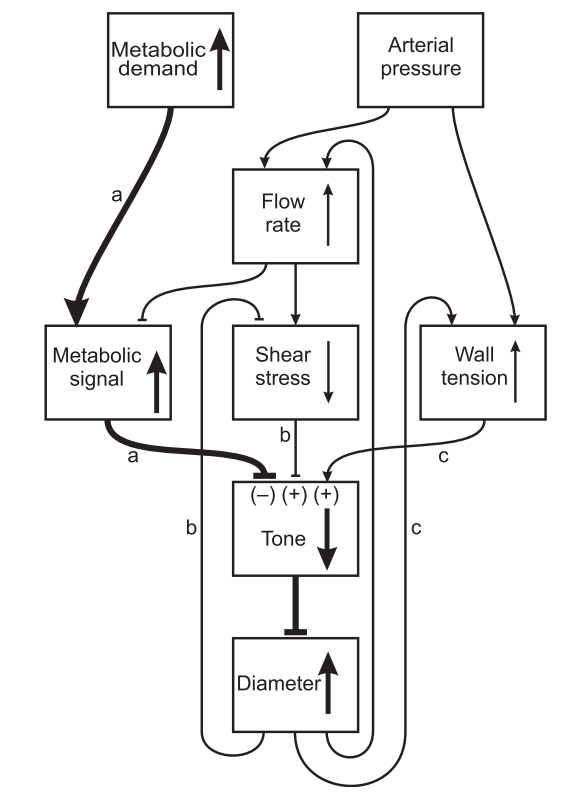
\includegraphics[width=.9\textwidth]{SummaryAutoregulationPathways}
  \caption{Summary of the activation pathways to autoregulation, taken from Arciero et al~\cite{Arciero_2008}. The tone compartment represent the activation of the smooth muscle cells on the vessels walls. (+) and (-) signs represent increase and decrease in tone of those cells, respectively. Metabolic signaling corresponds to ATP release from venules that travels upstream to cause arteriolar vasodilation.}
  \label{fig:Autoregulation-Summary}
\end{figure}

While the previous model by Guidoboni et al.~\cite{Guidoboni_2014b} models varaible resistance with a phenomenological approach, Arciero et al.~\cite{Arciero_2013} chose to directly model the vascular response through the various mechanisms acting on it.
The mechanisms tringgering autoregulation included in this work are: pressure, shear stress on the vessel wall, metabolic response, local tissue concentration of carbon dioxide and neural stimuli.
The idea of the model was to investigate the implications of each autoregulation pathways, individually and collectively, in glaucoma.
Glaucoma is characterised by degenerations of the optic nerve and the retinal ganglion cell layer and is associated with impairments of the vasuclar system, both in the systemic and retinal~\cite{Hulsman_2007, Bonomi_2000}.

\break

In the studies presented before, the vasculature is represented in a simplified way, either as compartments with varying resistance and capacitance or generated following optimality principles.
However, owed to its intrinsic function, the retina can be easily observed \textit{in vivo}.
Retinal angiograms have highlighted the differences between individuals\emph{INSERT REF}.
Therefore, some groups tried to simulate haemodynamics in vascular trees segmented from retinal angiograms~\cite{Aletti_2016, Malek_2015, Liu_2009, Rebhan_2019}.
However, they are at the moment limited to small segments of the vasculature, therefore ignoring the effect of downstream capillaries and venules in the distribution of haemodynamic parameters.
Despite the limitations and difficulties, those work provide a framework to investigate oxygen delivery and stress associated with ageing in vasculature and tissue that may affect visual functions~\cite{Rickett_2010,Sim_2013,Wessel_2012}.

\subsubsection{Ageing and diseased retina}

The effects of age and disease on the vasculature can be readily observed and quantified on retinal angiograms.
In particular, vessel density and larger capillary-free areas in the inner retina have been related to severity of the disease in disease such as glaucoma, diabetic retinopathy (DR) and neovascular age-related macular degeneration (nAMD)~\cite{Al_Sheikh_2016, Rao_2020, Yuan_2020}.
Furthermore, in those diseases, the retinal cells appear affected by changes in the vasculature.
One reason is the reduced perfusion that creates ischaemia within the retina.
Retinal non-perfusion areas can be visualized on angiograms, however, the exact availability of oxygen in the tissue can hardly be measured \textit{in vivo}.
Additionally, with age, blood vessels tend to work at full capacity in term of blood flow.
This leads to first, the loss of autoregulaton capabilities and second more stress on the blood vessels and the tissue they are embedded in.
Mechanical stress and its relation to diseases can be investigated \textit{in silico}.
Rehban et al. proposed such a model based on segmented vasculature.
Their finite element approach uses very fine grid elements to embed vessels directly into a retina with varying mechanical properties according to the cell layer.
The combination of haemodynamics in a segmented vascular network and the embedding in tissue provide direct insight in the stress acting on the tissue and vessel walls for different subjects.
The vascular network of an healthy subject, a subject with DR and a subject with glaucoma were used for comparison.
The inlet flow for each case was scaled accordingly to the subject specifities.
The experiments showed important differences in wall shear stress between each groups, with diseased cases being subject to higher stress.
This was true for all vessel diameters.
Guidoboni et al. used their theoretical vascular network to investigate the range of intraocular pressure that patients suffering from low or high systemic blood pressure or loss of autoregulation function can wisthand with limited variation of retinal blood flow~\cite{Guidoboni_2014b}.




\begin{itemize}
\item Rebhan 2019: Glaucoma and diabetic retinopathy, haemodynamics and tissue strees
\item Flower 2001: choroidal blood flow and treatment of subfoveal neovsacularization (Might not be the best place to put it?)
\item A word on Harris 2013 and mathematical models of glaucoma (review).
\end{itemize}


\subsection{Anti-VEGF therapy}

\subsection{Laser treatment}

% \begin{spacing}{0.0}
\bibliographystyle{abbrvnat} % {ksfh_nat}
{\normalsize \bibliography{Haemodynamics_nAMD_DR}}
% \end{spacing}

\end{document}
